\chapter{Simulations}
\label{chap:simulation}
To illustrate the working principle of IDI and to examine the Signal-to-Noise  characteristics, different simulations were performed:

First, it was assumed that the object to be imaged consists of discrete emitters, each emitting monochromatic spherical waves with the same wavelength, but with a randomly chosen phase, and the speckle image on a pixelated detector was simulated by addition of the scalar electric fields and taking the squared magnitude for each pixel. To reduce the influence of this discrete sampling on the simulated speckle patterns, the simulation is performed at XX the resolution and downsampled, such that each data point is the result of 4x4 discrete calculations
In this configuration, the speckle images of a single particle with randomly positioned emitters inside (approximating a single particle imaging setup), a focal volume filled with randomly positioned (non intersecting) hard spheres consisting of randomly positioned atoms (approximating for example many spherical nano particles imaged simultaneously) as well as a crystalline structure with emitters positioned at within a lattice were simulated. In the first two cases, a small-angle regime was chosen and the reconstruction was performed in 2D and as a 1D radial profile. For the crystalline structure, a realistic lattice constant in the same order of magnitude as the K$\alpha$ wavelength moves the reconstruction out of the small-angle regime and a 3D reconstruction of the reciprocal space was performed.
Additionally, in these simulations the effect of under-sampling was studied.

Second, to examine the influence of the fluorescence lifetime and pulse width, a time-resolved simulation was performed.
The results were compared with the approximation, that the contrast is determined by the product of the different number of modes.

Ultimately, the results of these simulations were used the determine the feasibility of an experimental setup using IDI







\section{Time Independent Simulations}
In an infinite coherence time, stationary sources approximation, the simulation of the speckle pattern can be performed time independently the superposition of scaler electrical fields emitted with random phases. The simulation of the intensity at multiple discrete points can be performed in parallel using GPU acceleration, resulting in a simple and fast to evaluate model.







\subsection{Detector Effects}
\label{sect:chargesharing}
To simulate the influence of detector dependent charge-sharing and readout noise, an image degradation is performed: After Poisson sampling the simulated speckle image, for each photon an uniform random position within its pixel is chosen as the center of a Gaussian distribution with $\sigma$=0.1, pixel, similar to the size of the point spread function (PSF) for MPCCD detectors \cite{mpccd}.
The signal within each pixel caused by one photon is given by the integral over the Gaussian,
\begin{equation*}
	I(\Delta x,\Delta y)=\frac{1}{4} \left(\text{erf}\left(\frac{\sfrac{1}{2}-\Delta x}{\sqrt{2}
		\sigma}\right)+\text{erf}\left(\frac{\sfrac{1}{2}+\Delta x}{\sqrt{2} \sigma}\right)\right) \left(\text{erf}\left(\frac{\sfrac{1}{2}-\Delta y}{\sqrt{2}
		\sigma}\right)+\text{erf}\left(\frac{\sfrac{1}{2}+\Delta y}{\sqrt{2} \sigma}\right)\right)
\end{equation*}
with $\sigma$ the standard deviation of the Gaussian in pixels and $\Delta x$, $\Delta y$ the distance of the pixel to the simulated photon center. Afterwards, a Gaussian readout noise is added. The effect of this degradation on the spectrum is illustrated in \fref{fig:degrad}.



\paragraph{Photon counting}
As the relevant signal for the correlation analysis is the presence of fluorescence photons, but charge sharing and readout noise of the detector as well as the presence of photons caused by air scattering and straylight degrade this signal, different approaches  of preprocessing to reduce this degradation are compared:

\begin{itemize}[nosep]
	\item Using the raw signal
	\item Using the raw signal after applying a noise threshold.
	\item Discretization by closest possible combination of signal and scattering photons for each pixel
	\item Discretization by maximum likelihood
	\item Droplet algorithm
\end{itemize}
The noise thresholding is done with a threshold of three times the standard deviation of the detector noise. Considering possible combinations of signal and scattering photons by finding  $nE_{fluorescence}+mE_{excitation}$ with integer $n$, $m$ closest to the observed value and only using the signal photon number $n$ for the correlation could reduce the influence of scattering as well as charge sharing, but does not account for the different probabilities of signal and scattering photons. If the detector noise level, the point spread function due to charge sharing as well as the distribution of signal and scattering is known or can be estimated, a Bayesian classifier can be trained on synthetic data, which returns for each observed value on the detector the number of signal photons with the highest probability causing this value (\fref{fig:probs}) and the associated decision boundaries. Depending on the apriori probabilities and the detector characteristics, this maximum likelihood solution can differ from the closest combination. For comparison, the PSANA Photon algorithm, a droplet algorithm considering only the signal photons is used \cite{psana}. The disadvantage of most droplet algorithms is the more obscure effect on the correlations, as they influence the position of photons and usually consider only a single energy or require a much higher computational effort.  

\begin{figure}
	\centering
	\begin{subfigure}[b]{0.45\textwidth}
		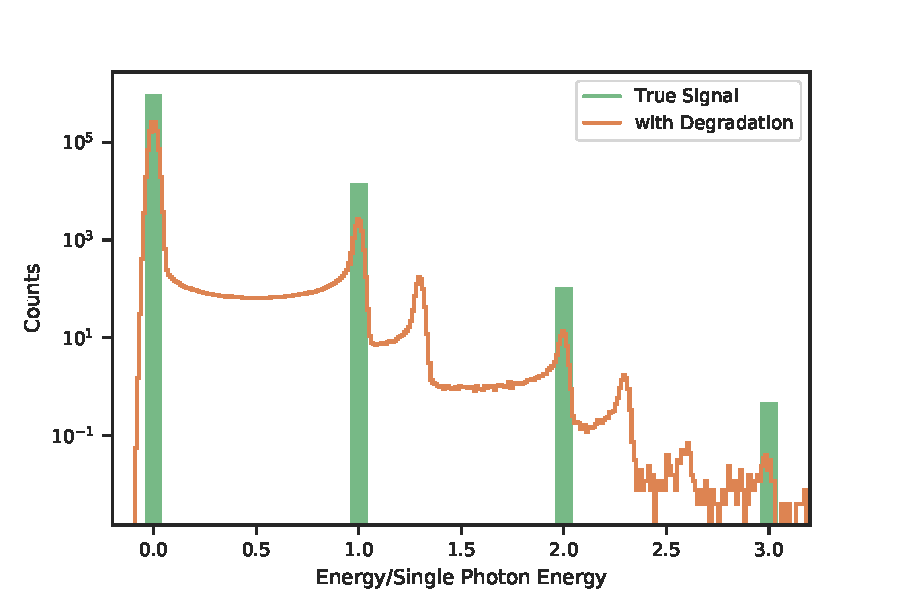
\includegraphics[width=\linewidth]{images/sharing.pdf}
		\caption{True histogram and degradation}
		\label{fig:degrad}
	\end{subfigure}
	\begin{subfigure}[b]{0.45\textwidth}
		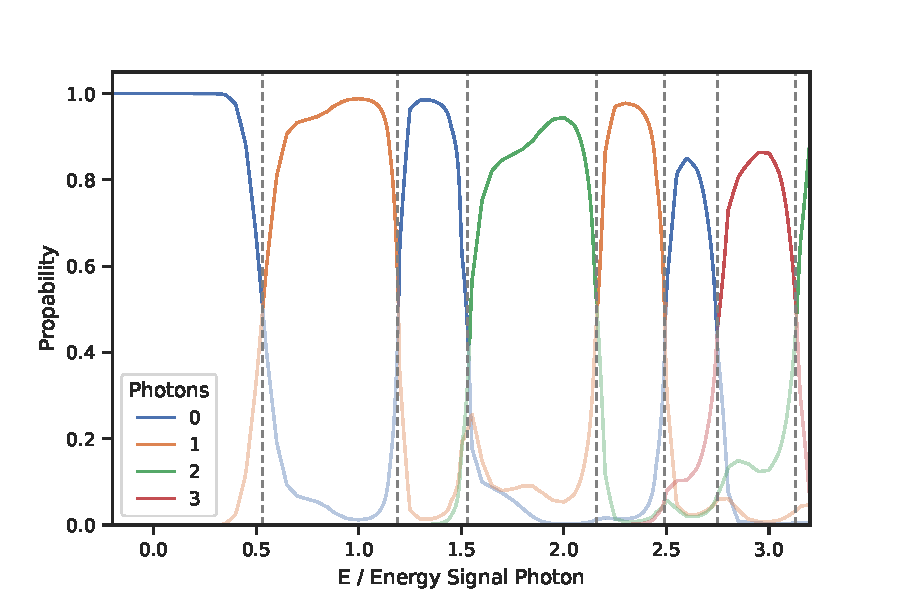
\includegraphics[width=\linewidth]{images/probs.pdf}
		\caption{Probabilities and decision boundaries}
		\label{fig:probs}
	\end{subfigure}
	
	\caption[Histogram, probabilities and decision boundaries for the photon number under the influence of charge sharing and noise]{For a Poisson distributed signal with mean 0.01 photons/pixel, a Poisson distributed scattering with mean 0.001 photons/pixel and an photon energy of 1.3 times the energy of a signal photon, a charge sharing PSF with $\sigma$ 0.1 pixel and a Gaussian noise with $\sigma$ 0.05 photons, the simulated histogram is shown on the left. Detector noise, charge sharing scattering photons degrade the histogram. The probabilities of an observed energy being caused by a certain number of signal photons is shown on the right, the dashed lines mark the decision boundaries for discrete signal photons of an Bayesian classifier.} 
\end{figure}


\begin{figure}
	\centering
	\begin{subfigure}[b]{0.85\textwidth}
		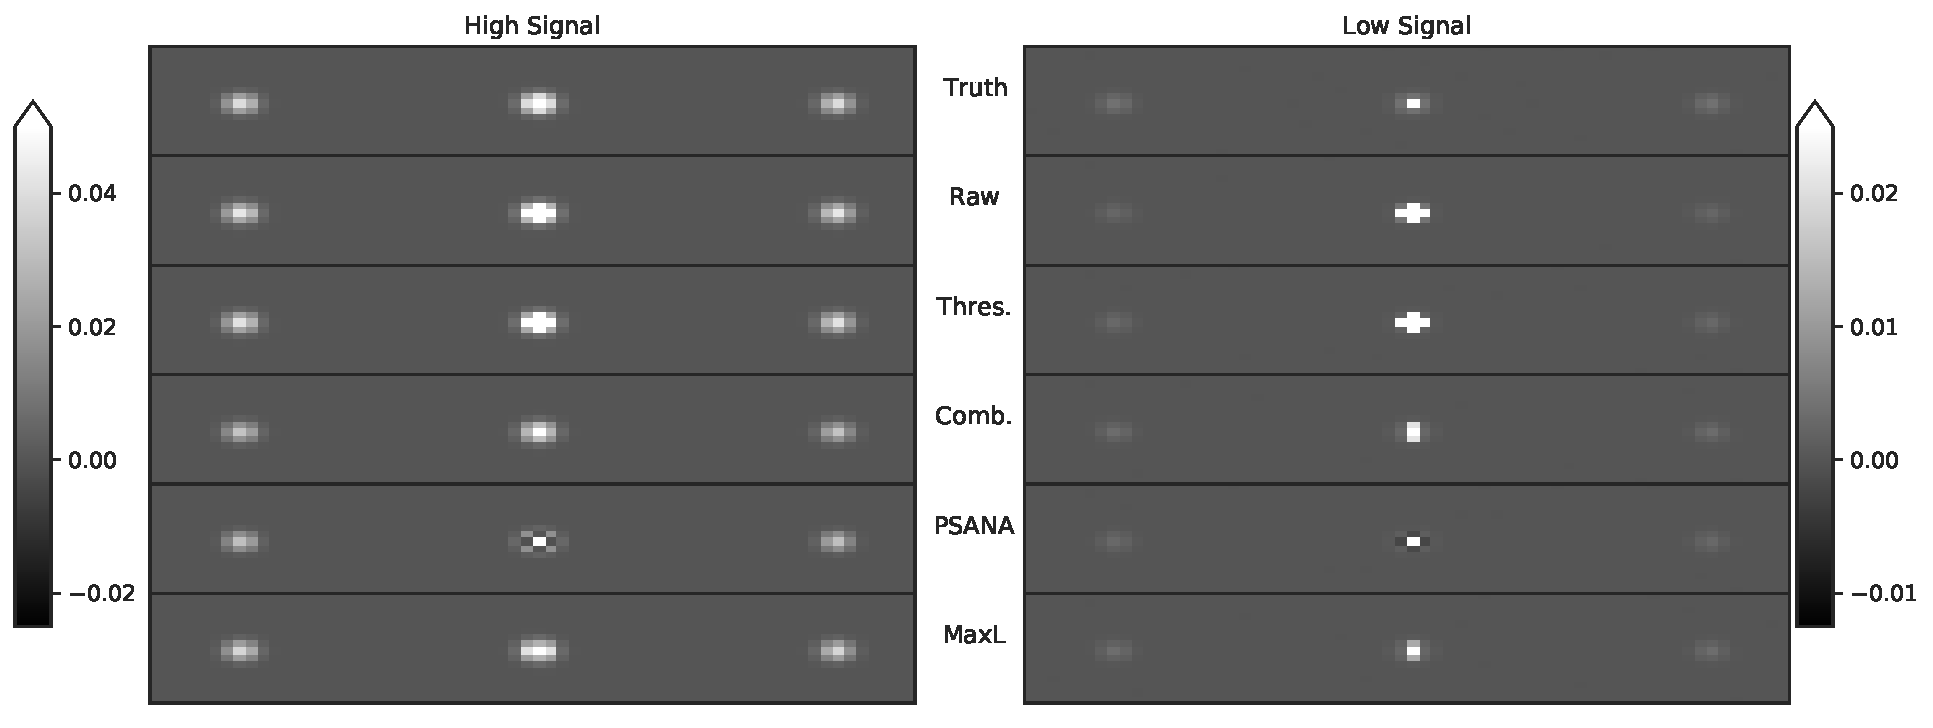
\includegraphics[width=\linewidth]{images/photonreconimg.pdf}
		\label{fig:photonreconimg}
		\caption{Center part of the reconstructions}
	\end{subfigure}
\\
	\begin{subfigure}[b]{0.95\textwidth}
		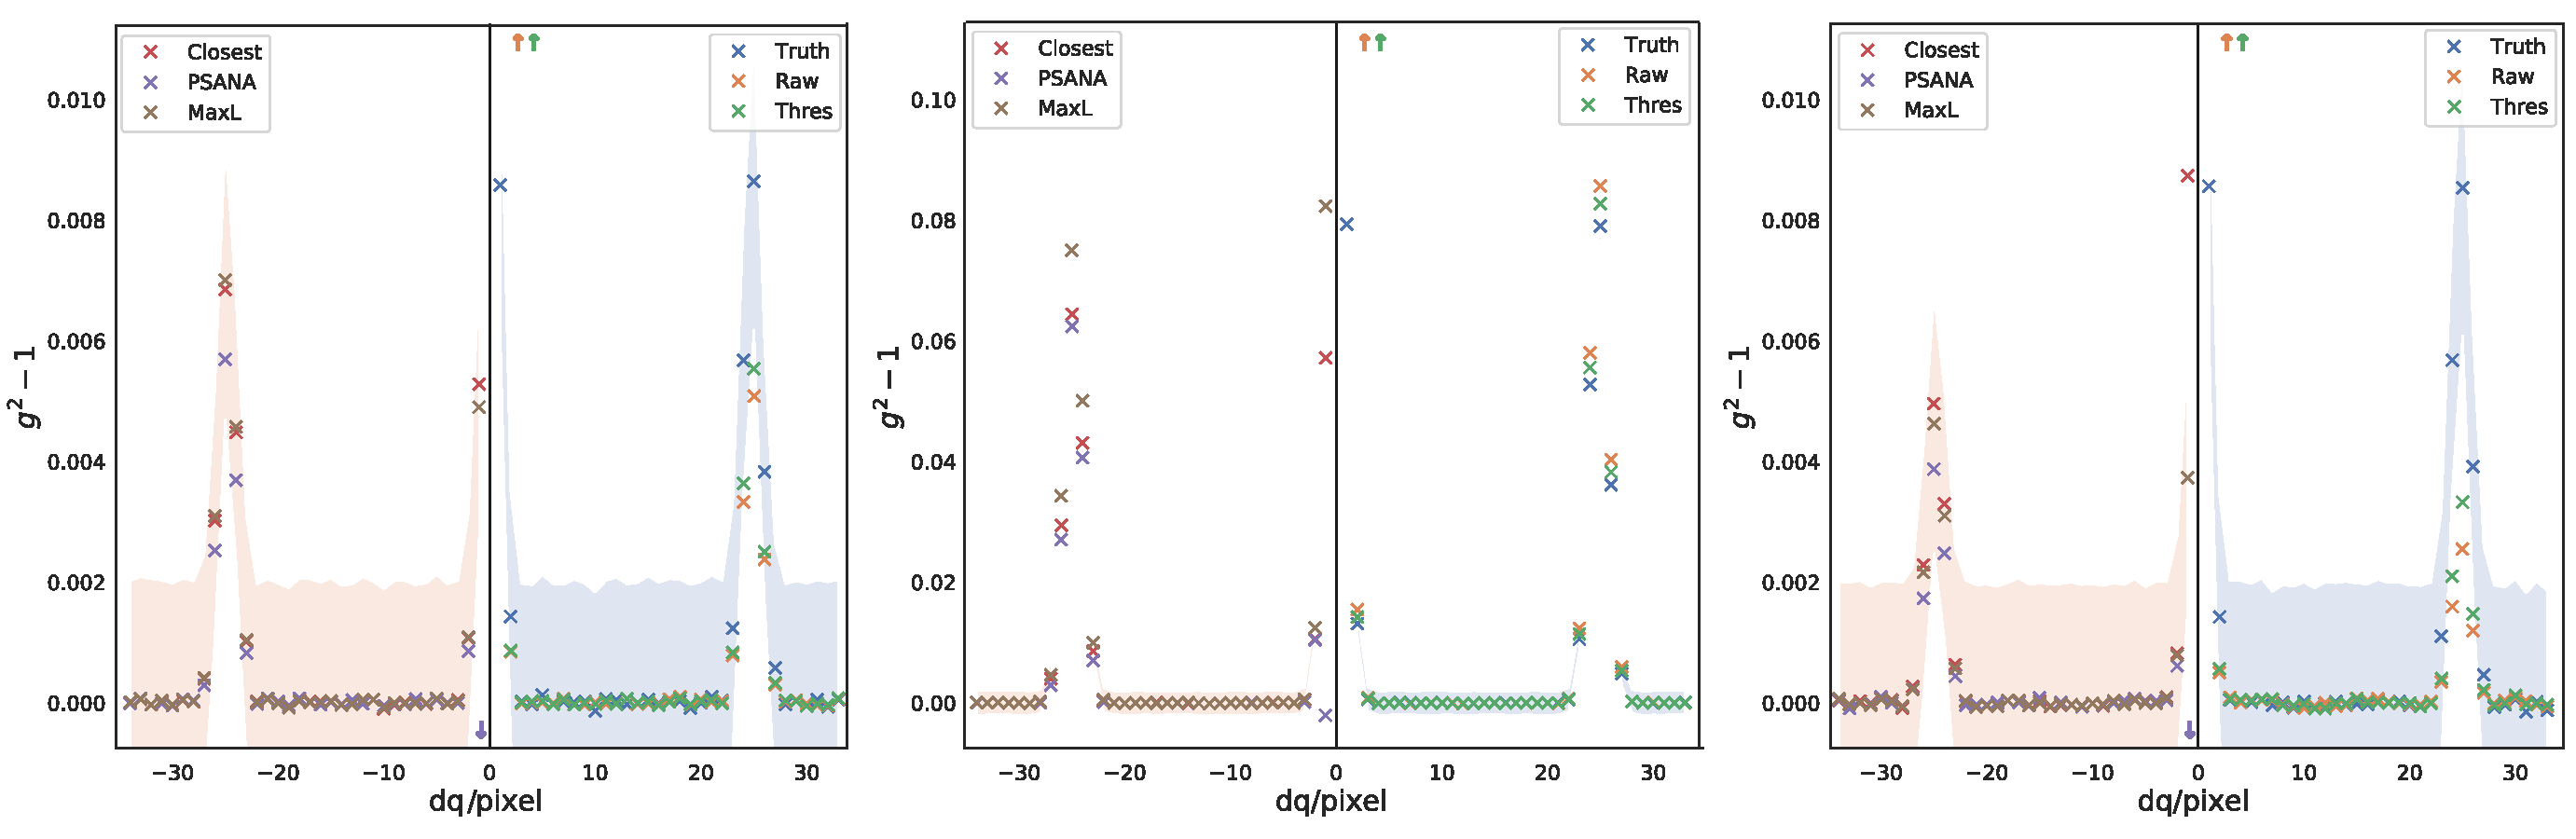
\includegraphics[width=\linewidth]{images/photonrecon.pdf}
		\label{fig:photonrecon}
		\caption{Line profiles}
	\end{subfigure}	
	
	\caption[Comparison of different photon counting methods for intensity correlation calculations]{Comparison of different photon counting methods for intensity correlation calculations: In \textbf{(a)} the center of the 2d results of the correlation for a simulated grating under two conditions are shown (high signal and low signal, parameters as described in the main text). In  \textbf{(b)}, for three different conditions (from left to right: high signal, low signal and high noise) line profiles are shown. Using the raw signal or simple thresholding overestimates the correlation between neighboring pixels, the PSANA droplet algorithm underestimates it compared to the ground truth. The maximum likelihood method and the "closest combination approach" reproduce the ground truth signal sufficiently well. For detailed quantitative results see also \fref{tab:photonrecon}.}
\end{figure}

To evaluate the different approaches, for a grating with pitch 50\,nm, line width 20\,nm and 100\,nm thickness in a 
400\,nm (FWHM) focus, resulting in $10^7$ excited atoms emitting at 10\,keV and a 1024x1024 pixel detector with 50\,um pixel size in 50\,cm distance, independent, 2000 florescence images are simulated. Three different cases are considered: With high signal ($10^5 $photons/image), low signal ($10^4$ photons/image), both having $10^3$ photons at 13\,keV as scattering noise and 500\,ev (gaussian) detector noise as a "high noise" case  with 2.5\,times the scattering and 2\,times the detector noise  ($10^4$ signal photons/image). Charge sharing is in all cases simulated with $\sigma$=5\,um. 
For each photon counting approach, reconstructions are performed in all the cases and compared to a reconstruction without noise or charge sharing as ground truth. For the first two cases, the center part of the reconstructions is show in \fref{fig:photonreconimg}, line profiles through the center and the first maximum for all cases are shown in \fref{fig:photonrecon}. In the different reconstructions, two effects are visible: In comparison with the ground truth, without any correction the reconstruction for low $q$ is be overestimated due to the correlation of neighboring pixels and underestimated for the first maximum (see \fref{tab:photonrecon} for detailed values). This can be slighlty reduced by thresholding, and greatly reduced by rounding to the closest combination as well as by the maximum likelihood classification. The PSANA droplet algorithm seems to join more neighboring photons than necessary, resulting in an incorrect negative correlation between neighboring pixels.  These observations in the simulation suggest using either the combination scheme or the classifier for an experiment, and both will be evaluated on the experimental data.

Possible avenues for improvement would be to use a more sophisticated droplet scheme based on error minimization allowing for subpixel resolution, incorporating the scattering photons into the droplet algorithm or using a neural network trained on synthetic images \cite{baumann2018,collaboration2014,schayck2020}


\subsection{Normalisation}
Mean of all pixels 
Mean of all pixels inside the overlap

If only a single image is taken, the expectation value for each pixel has to be approximated.

If multiple images are taken, under the assumption of ergodicity, the expectation value for each pixel can be approximated by its mean over many images. To account for fluctuations in the exciting FEL pulse and resulting fluctations of the fluorescence intensity, it can be assumed that the distribution over pixel intensities and FEL intensities are uncorrelated, and the detection probability of each pixel in each shot can be factorized into the product of the probability to detect a photon in a pixel and to detect a photon in a shot. Therefor, the effect of the FEL intensity fluctuations can be suppressed by normalizing each image by the total intensity of the image.



\subsection{Autocorrelation}

\subsection{Accessible Reciprocal Space}
	\paragraph{Accessible Reciprocal Space}
	As IDI is based on $g^2(\Delta \vec{q})$, for a ...  $q$ determined by the experimental geometry ($k$, detector size and distance), IDI can achieve higher $\left|\vec{q}\right|$ than a scattering setup, increasing the numerical aperture and could in theory be used to achieve a higher resolution. In practice, for most samples the resolution will be limited by the $q^{-4}$ dependence of $S$ and the SNR, thus only increasing the resolution for samples with strong features at high $q$.
	
	Compared to CDI, which measures $\vec{q}$ on the Ewald sphere and gives only limited $q_z$ information, IDI with a flat detector can give access  to a three dimensional volume in reciprocal space, as shown in \fref{fig:accesibleq} and, with greater $q_z$ coverage the greater the curvature of the Ewald sphere is. This, for example, gives access to multiple Bragg peaks in a single crystal experiment as shown in \fref{fig:accesiblebraggq}. 
		
	
	\paragraph{Detector Size and SNR}
	
	To asses the influence of the number of pixels of an detector (and correlation pairs) on the SNR, a simulation for a 1\,um thick Copper foil in an 100\,nm FWHM focus is performed. The detector size was varied from 64x64 to 3072x3072 pixels and always placed at the same distance of 1\,m, keeping the mean photon count per pixel constant. For the SNR calculations, the signal is defined as, the noise as the standard deviation XXX
	As show in \fref{fig:SNRdetsize}, under these conditions, the SNR is proportional to the square root of the number of pixels of the detector.



\begin{figure}[!htb]
	\centering
	\begin{tabular}[t]{cc}
		\begin{tabular}{c}
		\smallskip
		\begin{subfigure}[t]{0.4\textwidth}
			\centering
			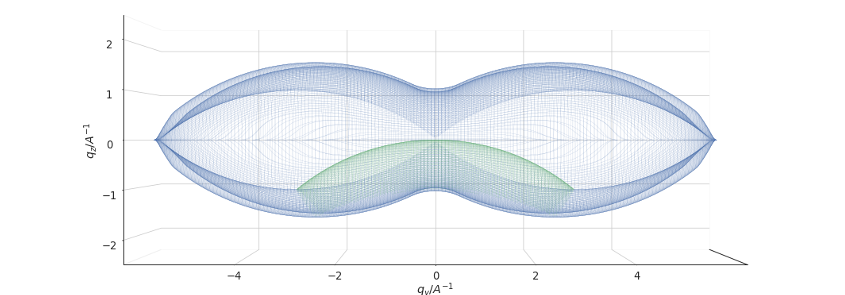
\includegraphics[width=0.9\textwidth]{images/accessibleq2.png}
			\caption{Accessible reciprocal space compared to CDI }
			\label{fig:accesibleq}
		\end{subfigure}\\
		\begin{subfigure}[t]{0.4\textwidth}
			\centering
			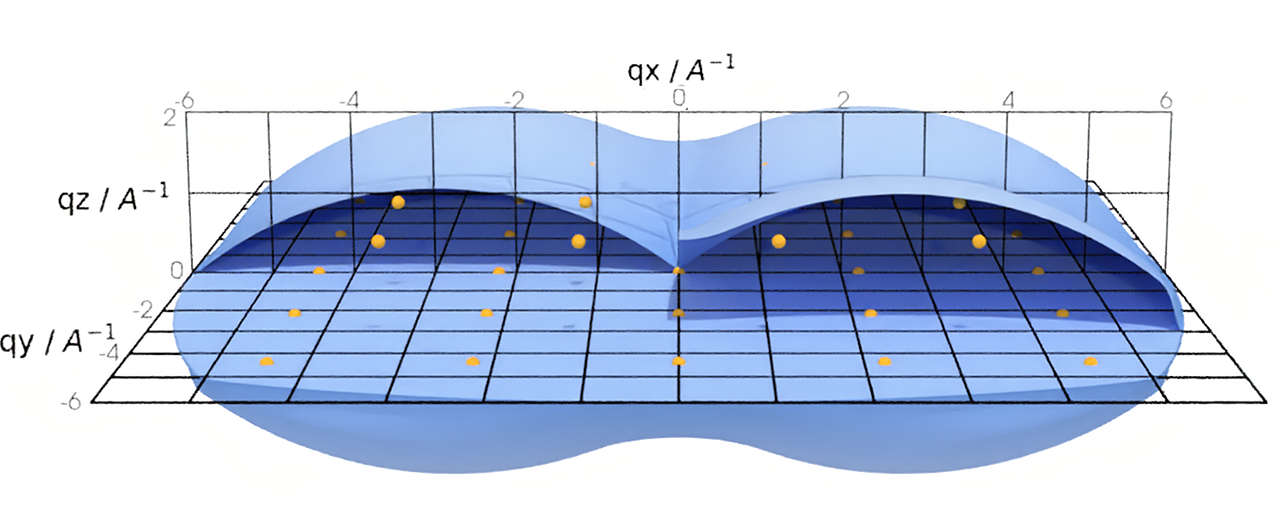
\includegraphics[width=0.9\textwidth]{images/accessibleq.png}
			\caption{Accessible reciprocal space with Bragg peaks}
			\label{fig:accesiblebraggq}
		\end{subfigure}
	\end{tabular}
		& 
	\begin{subfigure}{0.55\textwidth}
	\centering
	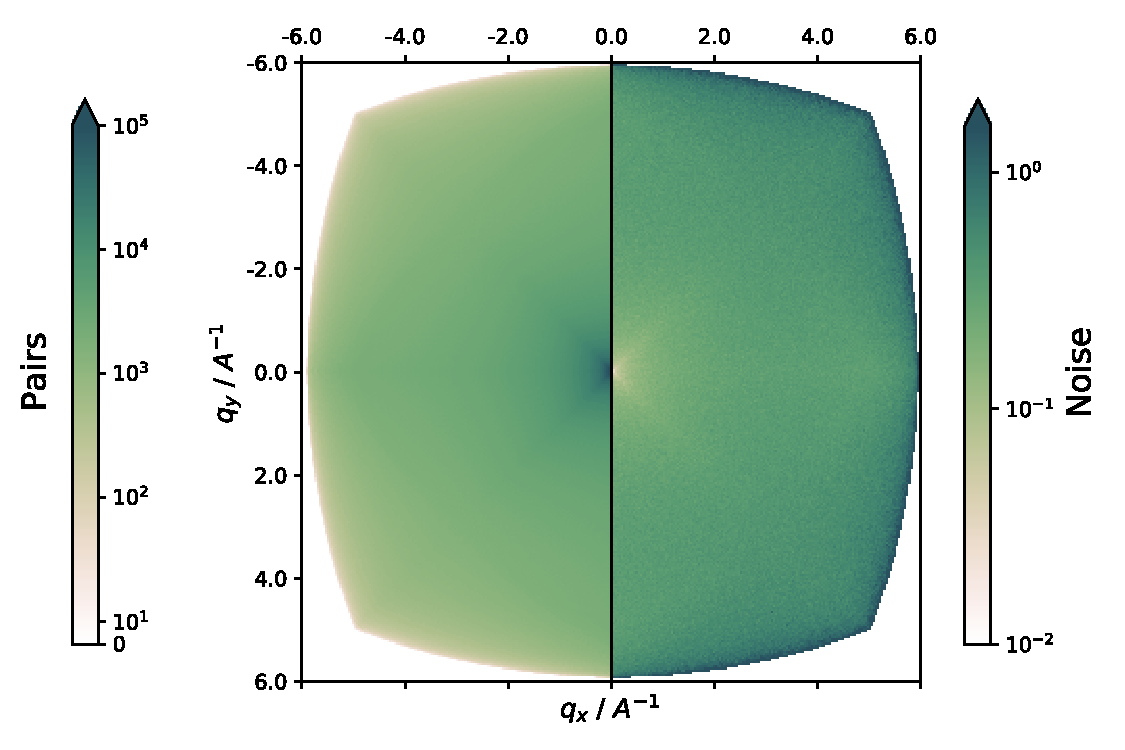
\includegraphics[width=0.8\linewidth]{images/pairsnoise.pdf}
	\caption{Correlation pairs and noise dependence on $\vec{q}$ } 
\end{subfigure}\\
	\end{tabular}
	\caption[Accessible reciprocal space]{The accesible reciprocal space with an 2048x2048\,pixel (100\,um pixelsize) at 12.5\,cm distance and 9.2\,keV is shown in a) and b). In a), the surface of the Ewald sphere accessible in an diffraction experiment is shown in green for comparison. IDI allows a reconstruction of a three dimensional volume. The position of GaAs Bragg peaks inside this volume is shown in b). As the accessible $q_z$ is depended on $q_x$/$q_y$ and smaller the larger the latter two, in this setup a precise alignment of the detector with regard to the lattice planes if useful to be able to image the maximal number of peaks. Using a square, centered, planar detector with uniform pixelsize, the number of correlation pairs for resulting in the same $\vec{q}$ depends on $\vec{q}$ as shown in on the left of c) for a $q_z=0$ slice. The noise (calculated as the standard deviation over 100 independent simulations) is therefor also non-uniform, as shown on the right of c).}
	
\end{figure}



\subsection{Number of Images}
As shown in \fref{fig:SNRNimages}, the SNR scales with  the square root of the independent images. This will be used to estimate the number of shots necessary to achieve a SNR greater than three to be able to experimentally verify IDI as an imaging method.
 
\subsection{Number of Modes}
\begin{figure}
	\centering
	\begin{subfigure}[b]{0.4\textwidth}
		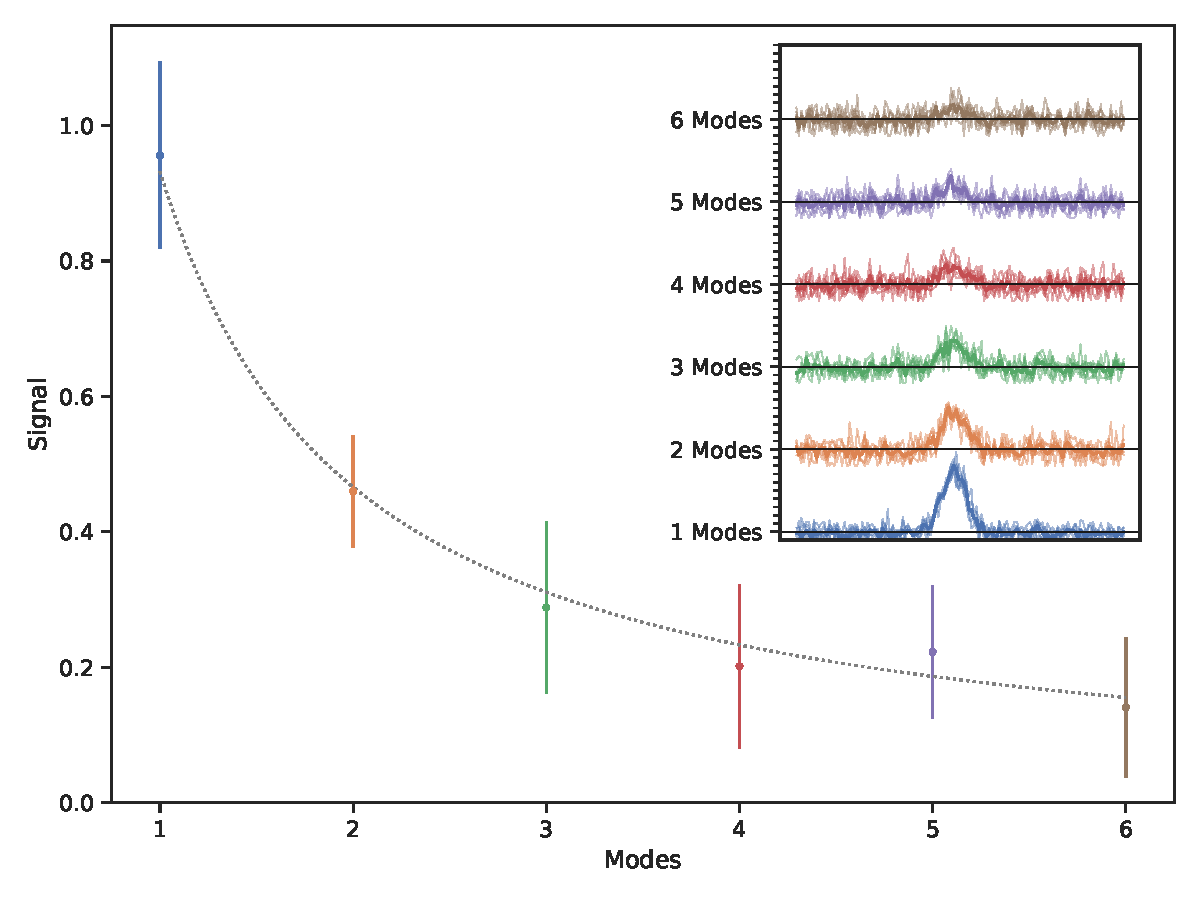
\includegraphics[width=\linewidth]{images/modes_signal.pdf}
		\caption{Signal dependence on number of modes}
		\label{fig:modes}
	\end{subfigure}
\end{figure}

\subsection{Undersampling and  Sample Size}


A simulation of a cubic single crystal with a simple cubic lattice of varying size (from 20$^3$ to 200$^3$\,atoms) is performed. The lattice constant is chosen as 5.7\,\AA, the fluorescence energy as 8\,keV. The simulated detector has 1024x1024 50\,µm sized pixels and is placed 8\,cm from the  sample. 
The simulation of the fluorescence patterns is performed with 4x4 oversampling (4096x4096 pixel) and rebinning to the detector size. Only a single coherence mode is simulated. The number of photons emitted by the sample in 4$\pi$ is chosen as equal the number of atoms in the sample. Hence, the mean number of photons per pixel is (especially for small crystal sizes) very small, but at the upper bound of an achievable photon yield in an experiment.

The peak signal-to-noise ratio is calculated by simulating 20-2000 independent images  and taking the mean intensity at the visible Bragg peaks positions as signal and the standard deviations at those positions over the independent simulations as noise, resulting in an estimated of the peak SNR of a single image.
Due to the low photon numbers, the Poisson noise is dominating the noise characteristic and with an increase in atoms in the focus, the SNR increases linear (as shown in \fref{fig:SNRNatoms}), up to the point where a the peaks are no longer fully sampled and the signal decreases linear with a further increase in the number of atoms in the crystal., resulting in a nearly constant peak SNR.
If instead of considering the peak value of the reconstruction as signal, the three dimensional integral over the Bragg peak would be considered as signal, the decreasing width of the Bragg peak with increasing size of the crystal would result in a nearly constant SNR under these low photon count conditions. 

This results suggests, that for an experimental verification using Bragg peaks, the excited volume of the crystal should be as large as possible without undersampling - for example choosing a thin single crystal and an appropriately tight focal volume.

\begin{figure}
	\centering
	\begin{subfigure}[b]{0.4\textwidth}
		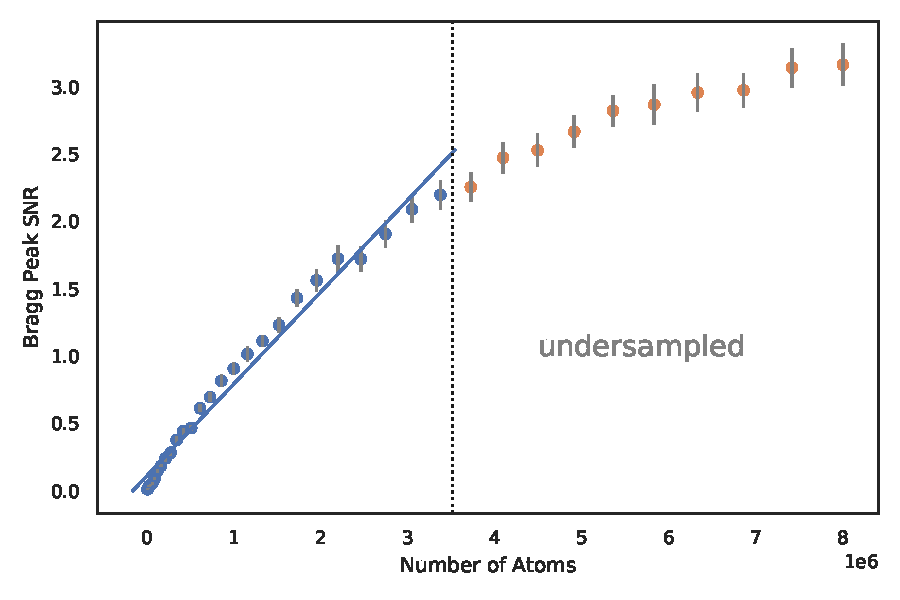
\includegraphics[width=\linewidth]{images/SNRNatoms.pdf}
		\caption{ SNR dependence on crystal size}
		\label{fig:SNRNatoms}
	\end{subfigure}
	\begin{subfigure}[b]{0.4\textwidth}
		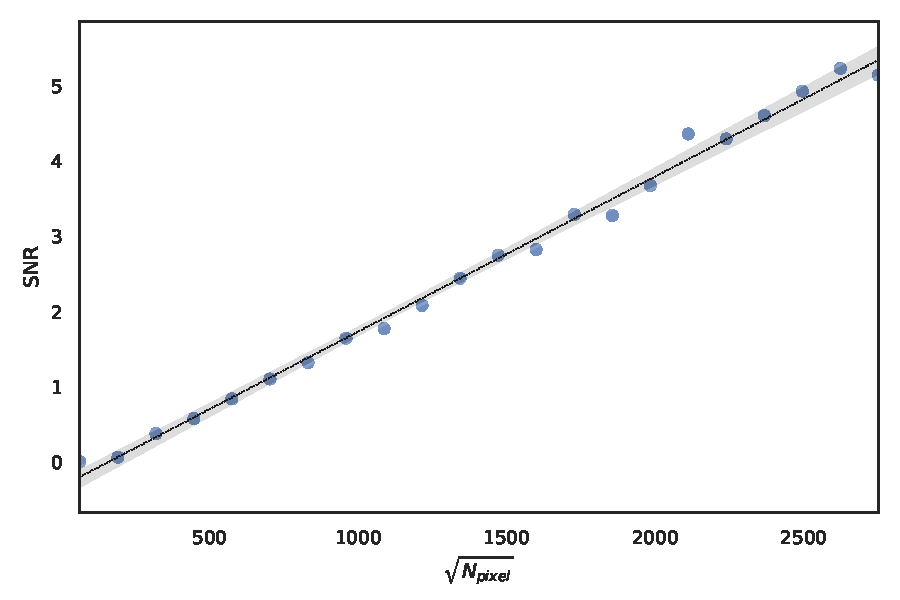
\includegraphics[width=\linewidth]{images/detsize.pdf}
		\caption{SNR dependence on detector size}
		\label{fig:SNRdetsize}
	\end{subfigure}
\caption[SNR dependence on crystal size and detector size]{SNR dependence on the crystal size (a): As the crystal size increases, the SNR increases linear (as shown by the linear regression) with the number of atoms in the sample as long as the Bragg peaks is sufficiently sampled (blue points), in undersampling conditions the signal strength decreases linear with the number of atoms resulting in a near constant SNR (right side of the dashed line). The error bars show the standard deviation of the SNR calculated for the 12 visible Bragg peaks. For details on the simulation parameters, see main text}

\end{figure}


%\subsection{Random Orientations}
%In an atomic resolution IDI experiment using a crystalline sample, there can be random orientations of the sample structure between each different shot if a powder is used as a sample.
%If a superlattice structure is used, it can be possible to limit the random orientations to orientations within a plane.
%The random orientations cause randomly oriented Bragg peaks and a significantly lower SNR as shown in \fref{fig:orientation}.  To have the best chance of experimental verification, a sample with static orientations between all shots used in the reconstruction is therefor beneficial.
%For random orientations in a plane and  imaging Bragg peaks of, it is possible to do an angular correlation of each reconstructed image and increase the SNR (as shown in \fref{fig:polarcor}), similar to a method in correlated X-ray scattering \cite{mendez2016}.




\subsection{Multiple Samples}
To decide if having more than one spherical sample in the focus is advantageous, an additional simulation is performed:
Multiple spheres inside the focal volume, placed randomly but ensuring a minimum distance between neighboring spheres larger than the diameter plus twice the thickness of an additional layer of non-fluorescing organic dispersion agent capping the spheres with no other interaction are simulated.  The number of particles is varied, ranging from a single sphere over multiple spheres to a Poisson Sphere Distribution as a random placement of particles with the minimal allowed spacing and mean a volume fraction of approx. 25\% \footnote{without the buffer layer, the volume fraction would be around 50\%, significantly smaller than the densest possible packing}. 
The structure factor of this ensemble of spherical particles is determined by three factors: The structure factor of the focus, the structure factor of points following an Poisson Sphere Distribution and the structure factor of a single sphere.(see \fref{fig:multisphere1}). As the number of spheres is increased, the influence of the focal volume increases and the distribution of the spheres's centers increases (see  \fref{fig:multisphere3})
For spheres with 20\, nm radius, a spacing layer of 5\,nm around each sphere, with  50000 excited atoms per sphere on average, a focus of 200nm (FWHM), the fluorescence on a 1024x1024 pixel (pixelsize 100\,um) detector placed 30\,cm is simulated. In this geometry, assuming constant distance to the sample for each detector pixel, approximately 1\% of the emitted photons reach the detector. 
For each number of spheres 5000 images are used for an IDI reconstruction (see  \fref{fig:multisphere2}).
As the number of photons sphere is kept constant, opposing effects occur:  With increasing number of particles, more are photons recorded and the Poisson noise is reduced, but the signal strength in low scattering angles is decreased as the structure factor changes from a single sphere to a hard-sphere model. Therefore, for the chosen simulation parameters an optimum in the detectebility of a correlation effect can be found for a medium number of samples in the focus.


As the number of particles inside the focus is increased, in the low $q$ region of the IDI reconstruction, the focal volume becomes more visible. For high numbers of particles, the structure factor of the distribution of the centers of the particles causes a reduction in the scattering factor in the low $q$ region. For low numbers of particles inside the focus, the Poisson noise casued by the low photon numbers dominates the error.


 
\begin{figure}
	\centering
	\begin{subfigure}[b]{0.32\textwidth}
		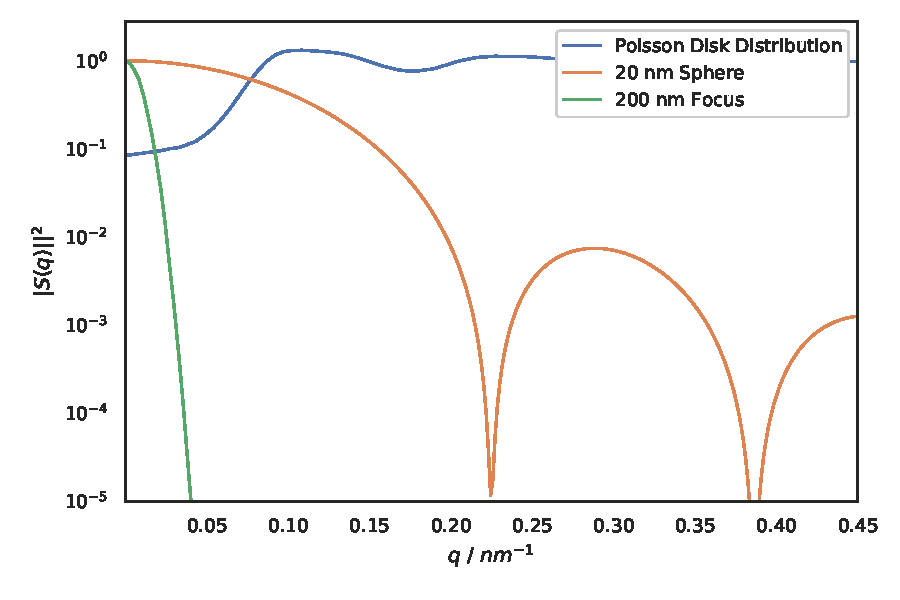
\includegraphics[width=\linewidth]{images/multisphere1.pdf}
		\caption{Structure Factors\\$ $}
		\label{fig:multisphere1}
	\end{subfigure}
	\begin{subfigure}[b]{0.32\textwidth}
		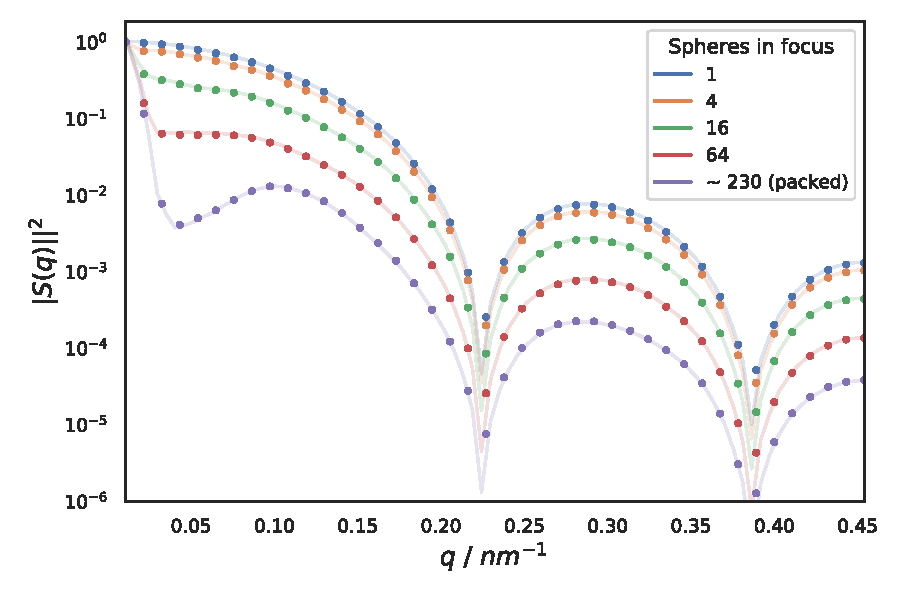
\includegraphics[width=\linewidth]{images/multisphere3.pdf}
		\caption{Structure Factor of Multiple Spheres}
		\label{fig:multisphere3}
	\end{subfigure}
	\begin{subfigure}[b]{0.32\textwidth}
		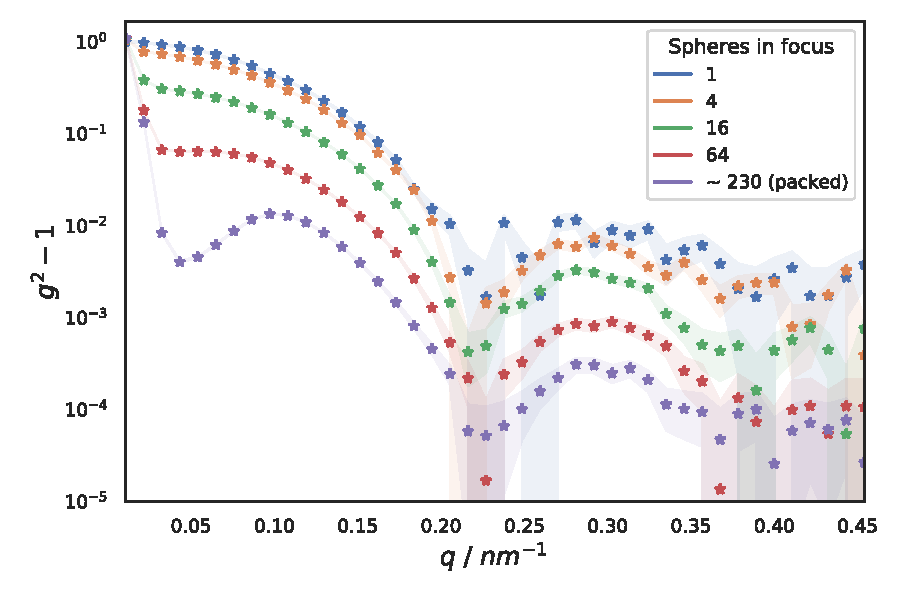
\includegraphics[width=\linewidth]{images/multisphere2.pdf}
		\caption{IDI Reconstruction \\ $ $}
		\label{fig:multisphere2}
	\end{subfigure}
\caption[Structure factors and reconstructions for multiple spherical samples]{Structure factors of a sphere with 20\,nm radius, a 200\,nm Gaussian focus and a random distribution of points at least 50\,nm apart (a), the structure factor of different numbers of hard 20\,nm radius spheres with an additional 5\,nm separating layer on each sphere inside the focal volume (b), and the result of an IDI simulation assuming iron fluorescence, a mean of $5*10^4$ excited atoms per sphere, a 1024x1024 pixel (100\,um pixelsize) detector in a distance of 30\,cm (resulting in approximately 1\% of the emitted photons being captured), and using 5000 images (c). The shaded area is the standard error of the mean over images, the markers show the discrete $q$ steps in the reconstruction.}

\end{figure}

\section{Time Dependent Simulations}
\label{sec:timedependend}
Each of the $N$ atoms is assigned an emitting time $t_{n}$ chosen according to the excitation pulse shape and its position. Starting from this emitting time, the atom emits an exponential decaying field with a decay time chosen to match the lifetime. 



For each discrete pixel on the simulated detector, for each atom the distance $d_n$, the arrival time $t'_n=t_n+d_n/c$ of each atom's initial radiance, and its time independent complex field $E_n=\frac{1}{d} e^{ikd_n+\phi_n}$ with initial random phase $\phi$ is calculated.
The time dependent E field is the summation over the decaying field of all atoms,
\begin{equation}
E(t)=\sum_{n=1}^N  E_n \Theta(t'_n  - t) * e^{-(t-t'_n )/\tau}
\label{eq:tdsum}
\end{equation}
and the simulated intensity the time integral over the magnitude squared of the E-field,
\begin{equation}
I=\int_0^\infty \left| E(t) \right|^2 .
\label{eq:tdint}
\end{equation}
To efficiently solve this integral for each detector pixel, it can be split into N parts with a constant number atoms which radiations have already arrived, and each of those parts can be solved analytically. For this, first all atoms are sorted by the arrival time at the pixel. At each arrival time $t'_n$, the sum in \fref{eq:tdsum} gets a new term and the field is calculated as
\begin{equation}
E(t_n)=E(t_{n-1})*e^{\sfrac{t_{n-1}-t_n}{\tau}}+E_n
\end{equation}
 This can be done with a parallel inclusive scan, as shown in \fref{algo:td}. This gives the supports for the integral, as show in \fref{fig:tdplot}, which can now be solved as
\begin{align}
	I&=\int_0^\infty \left| E(t) \right|^2 = \sum_{n=1}^{N-1} \int_0^{t_{n+1}-t_n} \left|E(t_n)\right|^2 e^{-2t/\tau} \dif t +\int_0^\infty \left| E(t_N)\right|^2 e^{-2t/\tau} \dif t \\
	 &=  \frac{\tau}{2}  \left|E(t_N)\right|^2 -  \frac{\tau}{2}\sum_{n=1}^{N-1} \left|E(t_n)\right|^2 (e^{-2 (t_{n+1}-t_n)/\tau} -1 ) 
\end{align}
This procedure is efficient in regards of discrete time steps that need to be calculated and can easily be run on a GPU.

\subsection{Influence of the Pulse Length}
For a sphere with 10\,nm radius consisting of $2*10^5$ atoms emitting 6.4\,keV fluorescence captured by an 256x256@50\,um detector in 20\,cm distance, the speckle strength (calculated as the standard deviation of the speckle pattern over the mean) of a series of simulations with different decay times $\tau$ of the emission and different FWHM of the exciting Gaussian pulse are shown in \fref{fig:tdpshere_specke}.  These follow the $1/\sqrt{erfcx(2\sigma/\tau})$ relation as predicted by the theory.  For each simulation, a reconstruction can be performed, resulting in radial profiles as shown for one $\tau$ in \fref{fig:tdpshere_recon}. The visibility of the reconstructions (\fref{fig:tdsphere_vis}) shows the for long pulses a reciprocal relationship.

\subsection{Influence of the Sample Thickness}
To investigate the influence of the sample thickness, the speckle strength in a second simulation is shown in \fref{fig:thickness}. In this simulation, a constant number ($10^6$) of 8\,keV emitters are placed inside a 200\,nm x 200\,nm (FWHM) Gaussian volume with varying thickness. To ensure sufficient sampling of the speckle pattern, the axis of varying thickness is always set perpendicular to the detector. The 64x64 pixel (pixelsize 100\,um) detector is placed in 1\,m distance. The simulation is performed with 4x oversampling and rebinning in both directions. The varying angle $\alpha$ influences only the mean (for each emitter) of the 1\,fs FWHM Gaussian from which the emission is sampled without influencing the overall volume in which the emitters are placed. Therefore, the change in SNR is only caused by the finite coherence time $\tau=1\,fs$, not by a change of the speckle size. Furthermore, no shot noise is considered in the simulation.
This simulations show that in high angles the limited coherence length of the fluorescence reduces the speckle SNR for thick samples, whereas in small angles, the sample thickness does not influence the SNR: In the 0° limit, the thickness is in beam direction and the position of an emitter along this axis does not change the arrival time of its contribution the the speckle pattern.




 As a thicker sample gives more photons and therefore less Poisson noise, but a higher number of temporal and spatial modes, thus a lower expected lower speckle visibility, a simulation close to experimentally feasible parameters is desirable.



\begin{figure}
	   \centering
		\includegraphics[width=0.5\linewidth]{images/tdplot.pdf}
	\caption[Integration in Time Dependent IDI Simulation]{To illustrate the integration in the time dependent IDI simulation, the (normalized) scalar field at one point of the detector created by 10 emitting atoms with $\tau$=1\,fs and a pulse FWHM of 2\,fs is shown. The solid colors show each atom's field, the line plot the (phase correct) sum. The simplify the calculations, only the time points marked with stars are calculated. To solve the integral \fref{eq:tdint}, it's sufficient to calculated the squared magnitude at those points and to do a piecewise integration from each star-shaped marker the next dot-shaped marker. The color wheel in the top illustrates the phase encoding in the plot.}
	\label{fig:tdplot}
\end{figure}


\begin{figure}
	\centering
	\begin{subfigure}[t]{0.45\textwidth}
		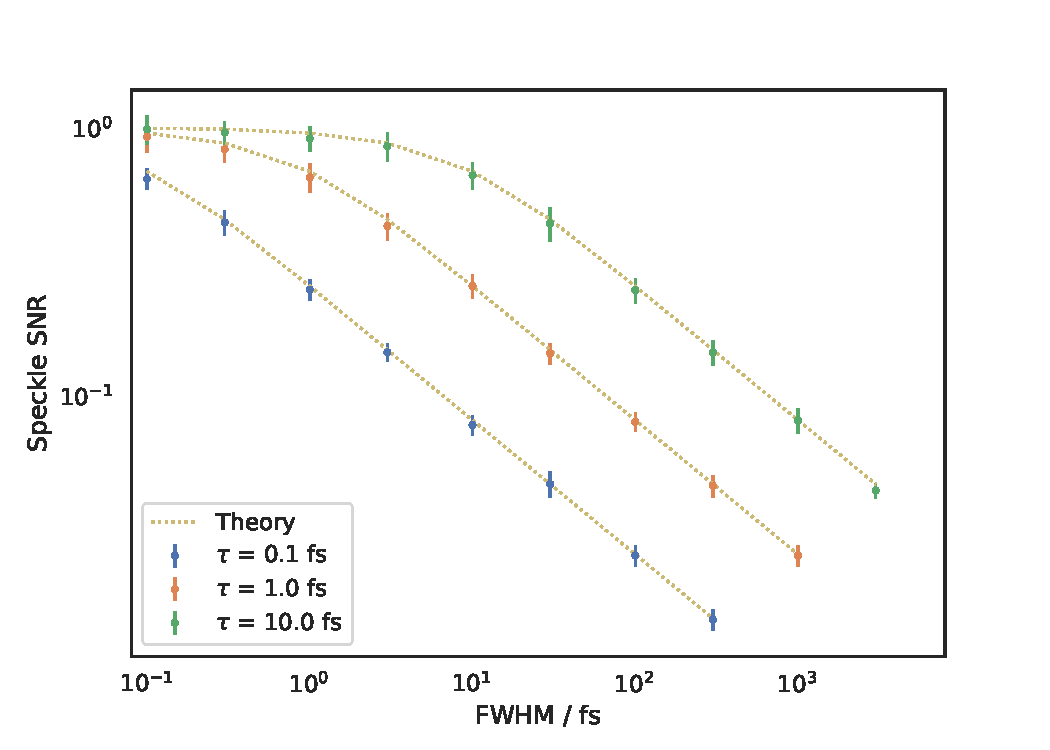
\includegraphics[width=\linewidth]{images/timedependent_1.pdf}
		\caption{Speckle SNR for different pulse FWHM and decay times $\tau$\\$ $}
	\end{subfigure}
	\hspace{0.1cm}
	\begin{subfigure}[t]{0.45\textwidth}
		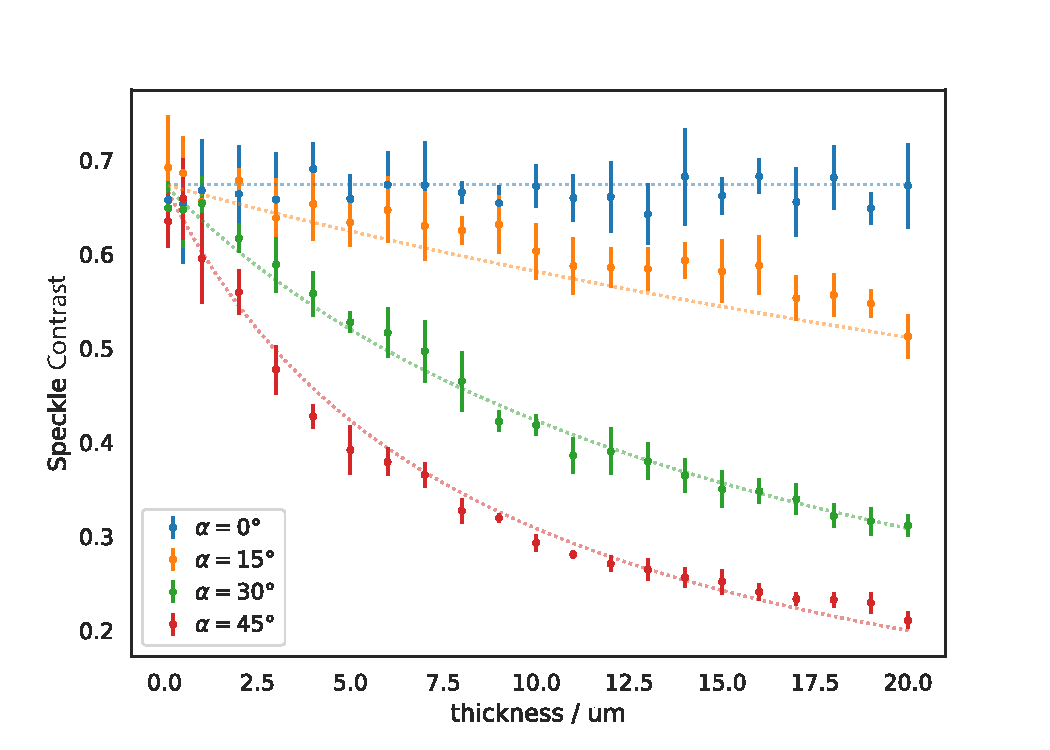
\includegraphics[width=\linewidth]{images/thickness.pdf}
		\caption{Speckle SNR for different sample thicknesses and angles}
	\end{subfigure}
	\caption[Speckle SNR in Time Dependent Simulation]{ In a) the SNR of the simulated speckle pattern for different pulse length and decay times $\tau$ of a spherical object is compared with the theoretical dependence on the ratio of pulse length and $\tau$ (details in text), showing good agreement. In b) the influence of sample thickness on the speckle SNR under different angles is show (using the mean of 5 independent simulations and the standard deviation as errors). The dashed lines are $y=c/\left(1+(\sfrac{\sin^2 \alpha}{4})\right)$ regressions. For small angles, the sample thickness does not influence the SNR.}
\end{figure}
\begin{figure}
	\centering
	\begin{subfigure}[b]{0.45\textwidth}
		\centering
		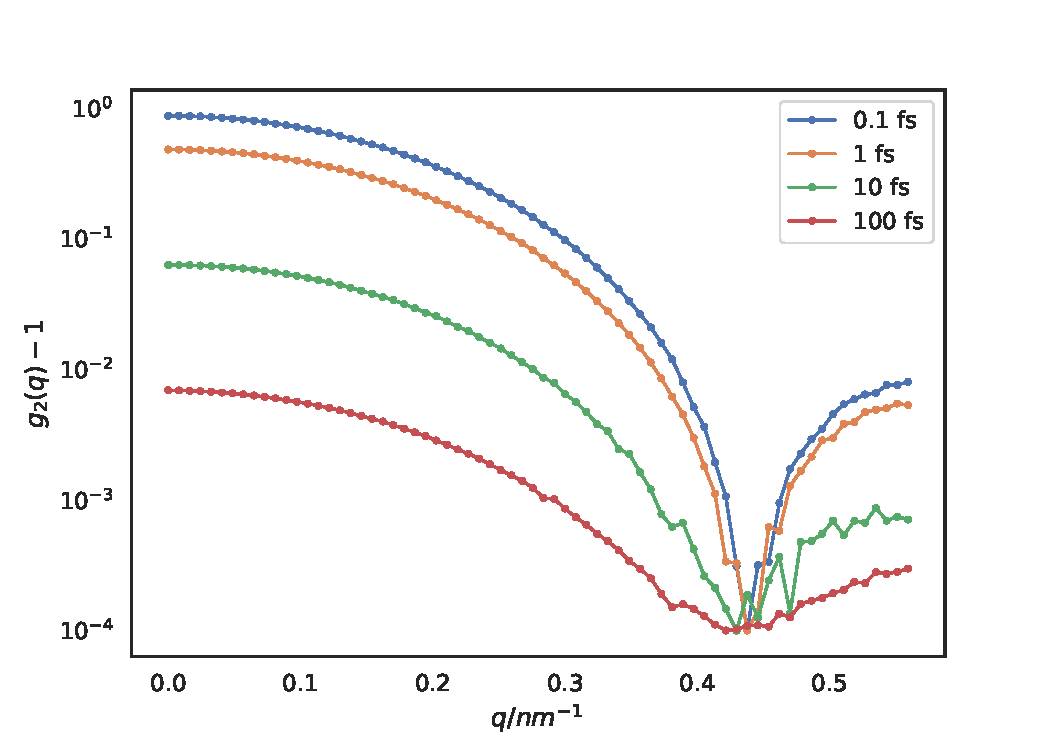
\includegraphics[width=\linewidth]{images/tdsphere.pdf}
		\caption{Reconstructed radial profiles at different pulse FWHM and fixed $\tau = 0.1$\,fs}
	\end{subfigure}
	\hspace{0.1cm}
	\begin{subfigure}[b]{0.45\textwidth}
		\centering
		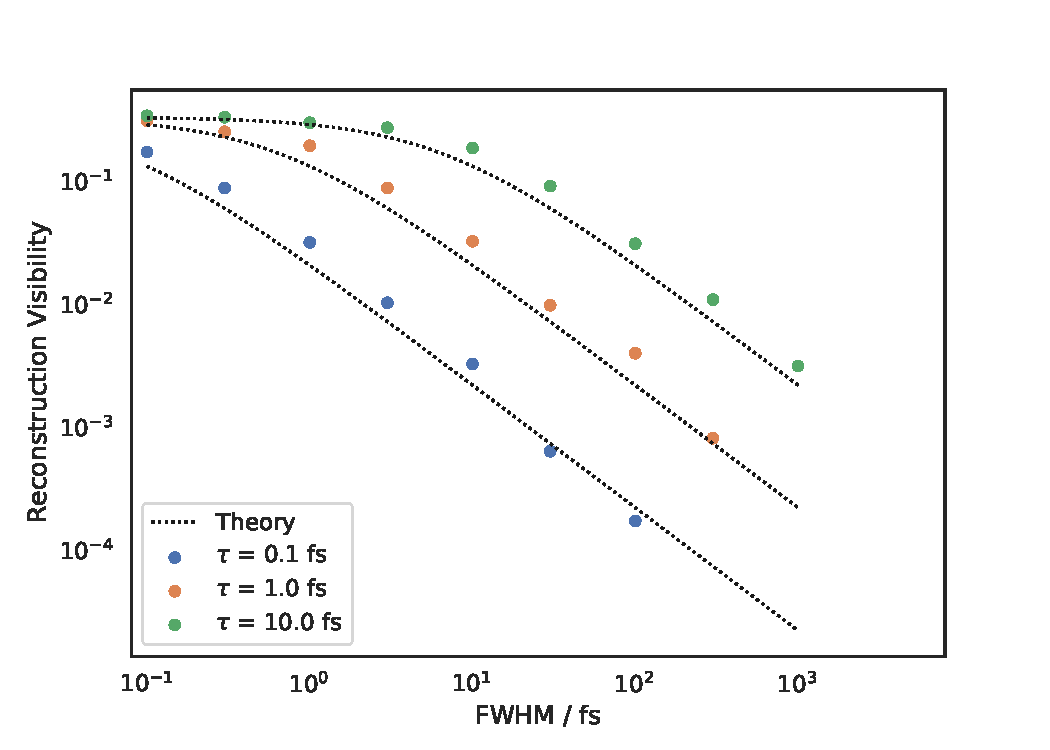
\includegraphics[width=\linewidth]{images/timedependent_2.pdf}
		\caption{Visibility of the reconstruction for different pulse FWHM and decay times $\tau$}
	\end{subfigure}

	\caption[Reconstruction Time Dependent IDI Simulation]{In a) exemplary radial profiles of the reconstruction of 50 images simulated for a spherical object are shown for one fixed $\tau$. Those reconstructions are used to plot the  dependence of the visibility on the pulse width in b). For long pulses, the reciprocal dependence on the pulse length is visible.}
	\label{fig:tdpshere}
\end{figure}




\section{Implications for an experimental design}

The result of a simulation for a thick 5\,um Copper foil, rotated 45° with respect to the beam (200\,nm focus FWHM, 10\,fs pulse FWHM), measured with an detector with 50\,um pixel size (charge sharing $\sigma$=5\,um) placed in a distance of 1\,m  perpendicular to the beam is shown in \fref{fig:simfoil}. Even tough the under sampling in the horizontal direction, causes an significant reduction in signal strength, ~100 images suffice in the simulation to get an acceptable SNR to clearly see the  focal size, leading to the estimation that even with additional noise sources, less than 1000 images might suffice for an experimental verification.

\begin{figure}
	\centering
	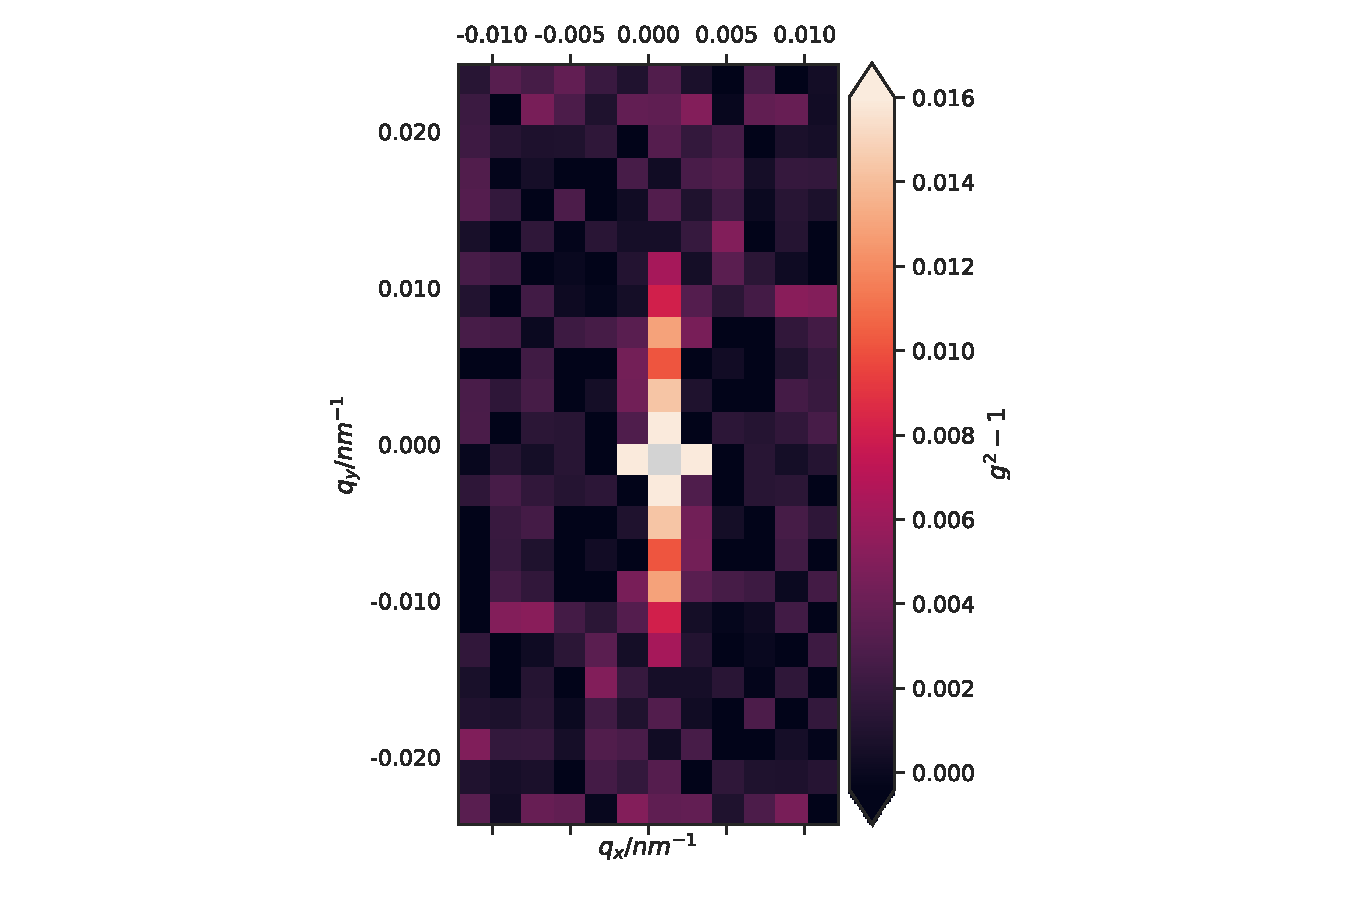
\includegraphics[width=0.5\linewidth]{images/sim_foil5umCu_shared.pdf}
	\label{fig:simfoil}
	\caption[Simulation of a metal foil with similar parameters as used in the experiment]{Simulation result for a metal foil placed in a 200\,nm focus viewed perpendicular to the incoming FEL beam. No correction for charge sharing is applied. The center pixel is masked, as $g^2(0)-1\approx 
		\frac{1}{M}+\frac{1}{\mu}$ is dominated by the mean count and does 
		not carry spatial information.}
\end{figure}

